\section{Beam Source Assembly Procedure}
\label{source_assembly_appendix}

\begin{enumerate}
   \item Install PT815 and PT415 into beam source
   \item Put beam source on its stand (at/near final position)
   \item Disentangle the temperature sensors and heaters
   \item Clean the new screws
   \item Attach PT warm and cold stage thermometers
   \item Install 40K shield
      \begin{enumerate}[label=\Alph*.]
         \item Attach 3/8-16 threaded rods to the vacuum chamber top plate
         \item Attach 40K flexible braided heat links to the PT warm stages
         \item Assemble 40K box with bottom plate
         \item Attach the neon heat exchanger to 40K top plate.
         \item Attach 40K top plate to the 3/8-16 threaded rods
         \item Finish the neon line.
         \item Insert 40K internal structure
         \item Screw the 40K flexible braided heat links into the 40K top plate
         \item Attach top plate to internal structure
         \item Attach the temperature sensor to 40K top \&\ bottom plates
         \item Adjust and fix the height of the 40K box.
      \end{enumerate}
   \item Add copper pieces
      \begin{enumerate}[label=\Alph*.]
         \item 4K top plate with 1/4-20 threaded rods and temperature sensor
         \item PT815 adapter
         \item Attach cell top plate to cell
         \item Install cell onto PT815 adapter
         \item Add cell heaters and thermometers
         \item Add snorkel, nozzle plate, input nozzle, back snorkel
         \item Connect the neon line: SS line, copper line
         \item Add remaining cell temperature sensors
         \item Add 4K side plates, bottom plate
         \item Add 4K bottom thermometer, cell heaters
         \item Add 4K flexible braided heat link
         \item Adjust the height of the 4K box
      \end{enumerate}
   \item Close the heat shields with the remaining plates.
   \item Add remaining feedthroughs. Test heaters, thermometers. Leak check.
   \item Attach helium lines, test cryogenic operation.
   \item Insert target.
\end{enumerate}

\begin{figure}[b]
    \centering
    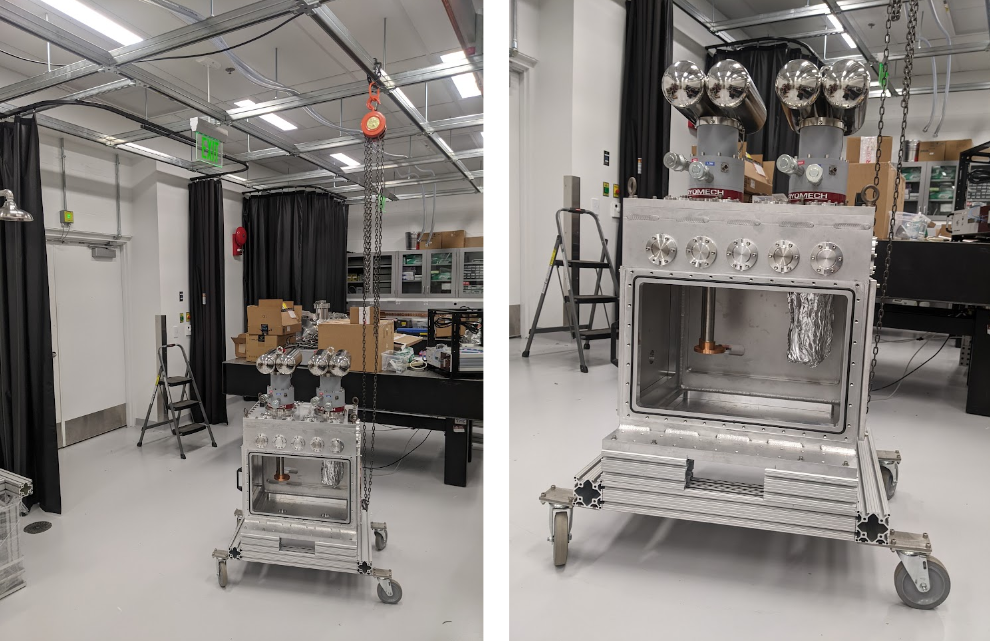
\includegraphics[width=\textwidth]{figs/todo/assembly/1.png}
    \caption[Step 1: return PTs to vacuum chamber.]{Step 1: return PTs to vacuum
    chamber. Very important: make sure each pulse tube is in its own correct
    hole. PT815 is towards the front of the box, and PT415 towards the back. The
    holes are not interchangeable, the vacuum chamber is not symmetric!}
    \label{beam_source_assembly_1}
\end{figure}

\begin{figure}
    \centering
    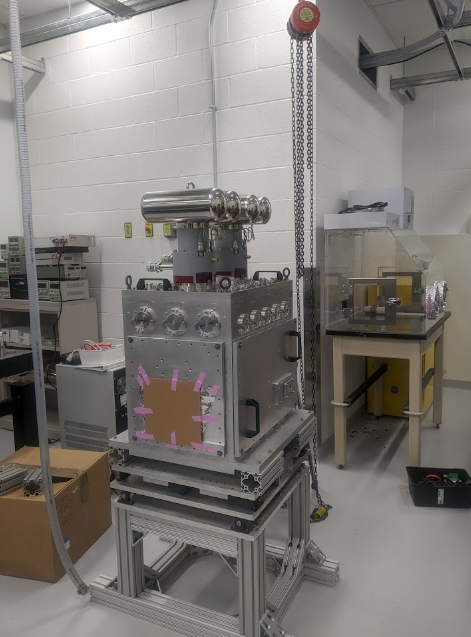
\includegraphics[width=.5\textwidth]{figs/todo/assembly/2.png}
    \caption{Step 2: return BS to 80/20 frame.}
    \label{beam_source_assembly_2}
\end{figure}

\begin{figure}
    \centering
    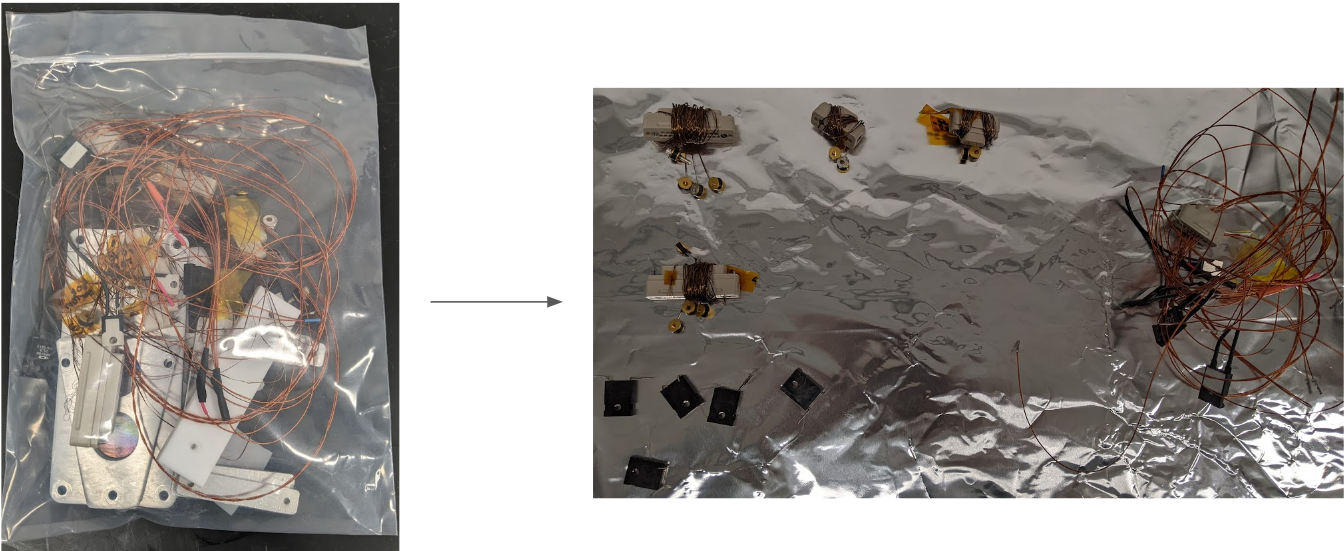
\includegraphics[width=\textwidth]{figs/todo/assembly/3.png}
    \caption{Step 3: disentangle internal electronics.}
    \label{beam_source_assembly_3}
\end{figure}

\begin{figure}
    \centering
    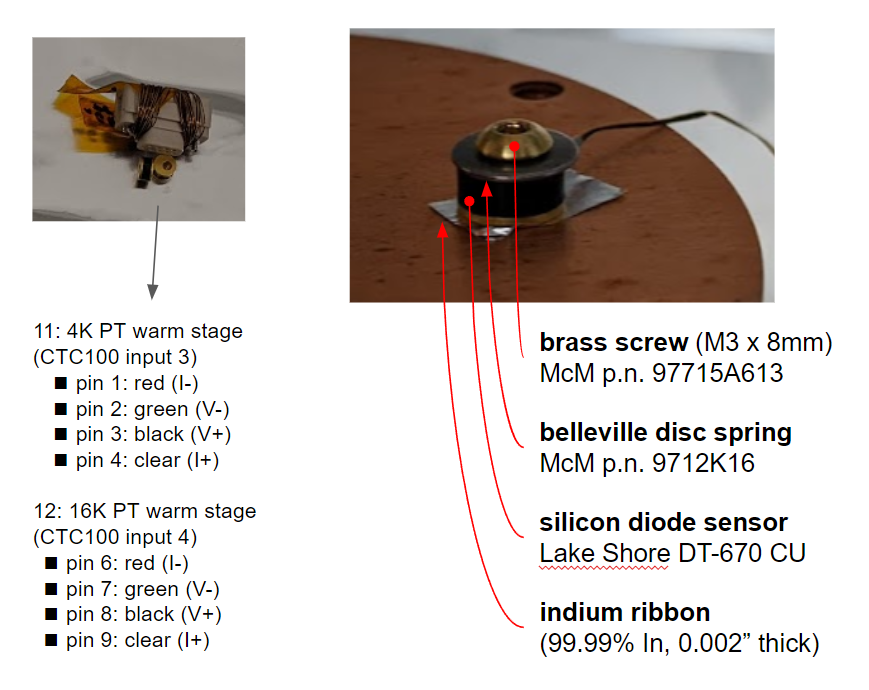
\includegraphics[width=.8\textwidth]{figs/todo/assembly/5A.png}
    \caption{Step 5A: attach PT warm-stage thermometers.}
    \label{beam_source_assembly_5A}
\end{figure}

\begin{figure}
    \centering
    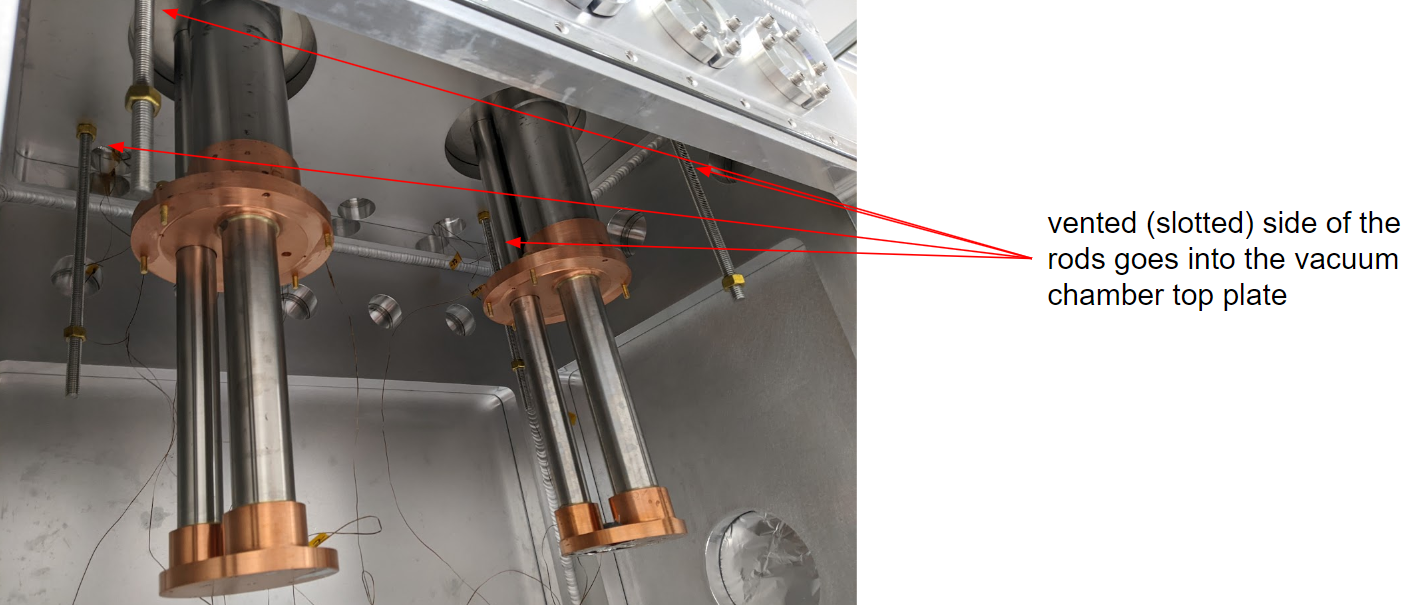
\includegraphics[width=\textwidth]{figs/todo/assembly/6A.png}
    \caption{Step 6A: 3/8-16 threaded rods.}
    \label{beam_source_assembly_6A}
\end{figure}

\begin{figure}
    \centering
    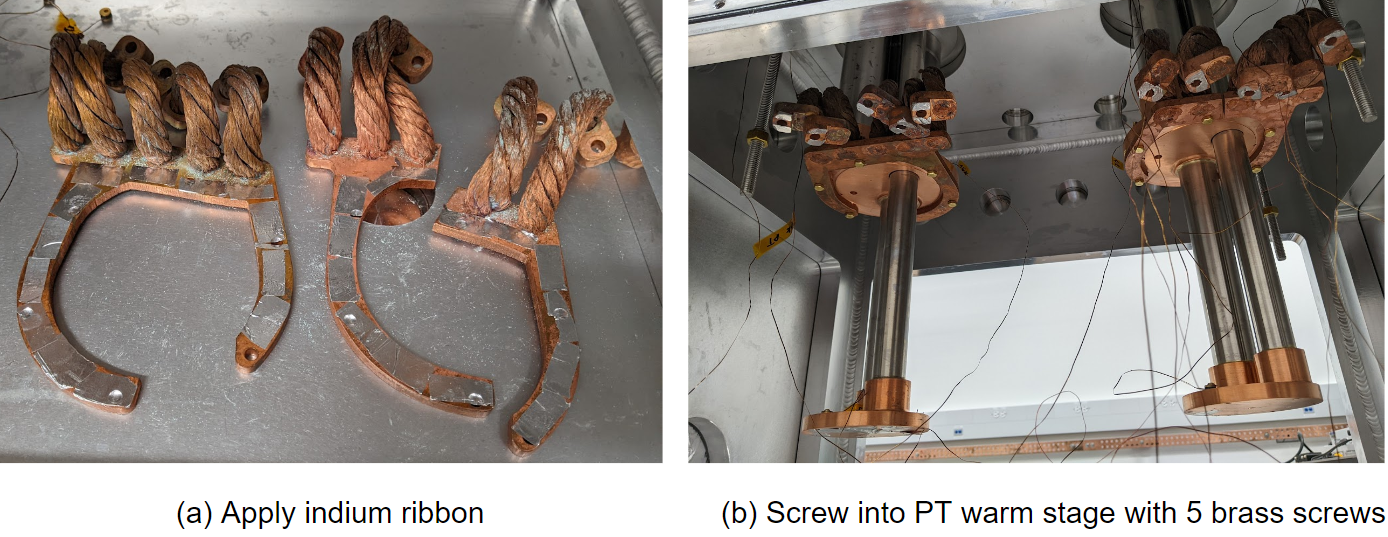
\includegraphics[width=\textwidth]{figs/todo/assembly/6B.png}
    \caption[Step 6B: 40K heat links to PT.]{Step 6B: 40K heat links to PT. NB:
    flexible links must face away from ablation laser!}
    \label{beam_source_assembly_6B}
\end{figure}

\begin{figure}
    \centering
    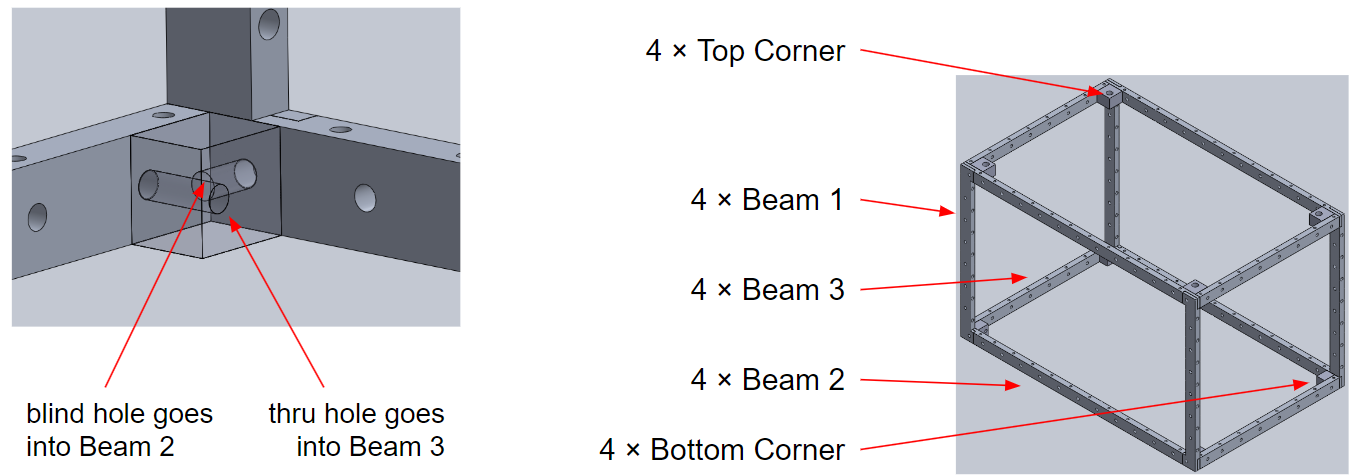
\includegraphics[width=\textwidth]{figs/todo/assembly/internal.png}
    \caption{40~K shield internal structure.}
    \label{beam_source_assembly_internal}
\end{figure}

\begin{figure}
    \centering
    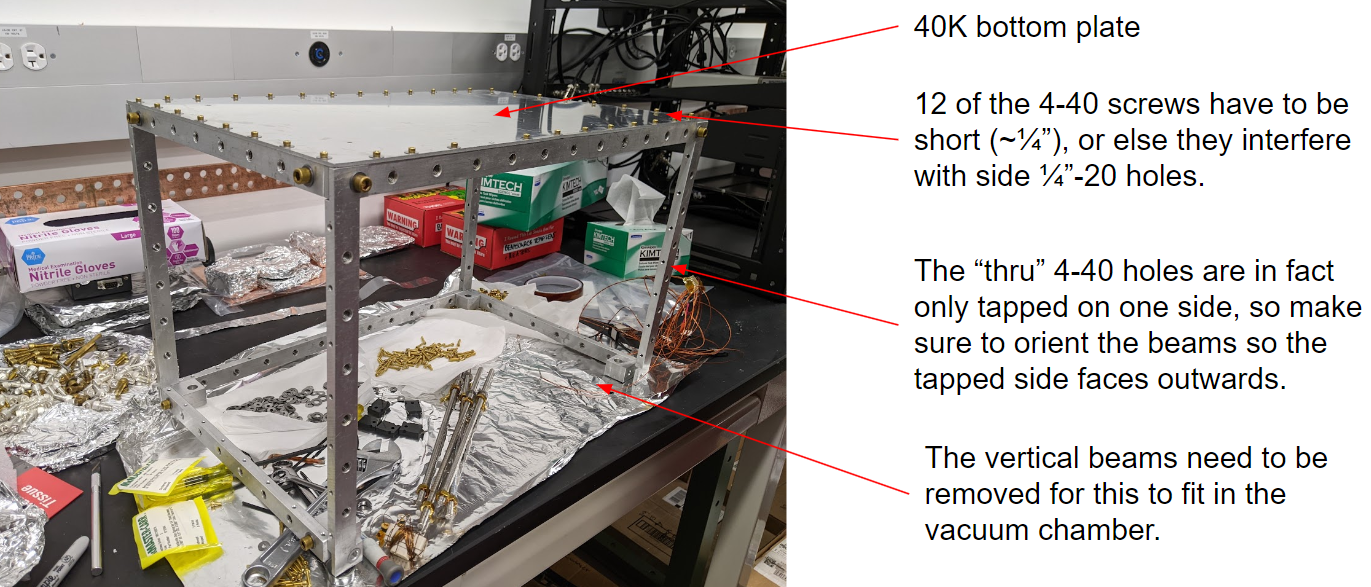
\includegraphics[width=\textwidth]{figs/todo/assembly/6C.png}
    \caption{Step 6C: Assemble 40K box w/ bottom plate.}
    \label{beam_source_assembly_6C}
\end{figure}

\begin{figure}
    \centering
    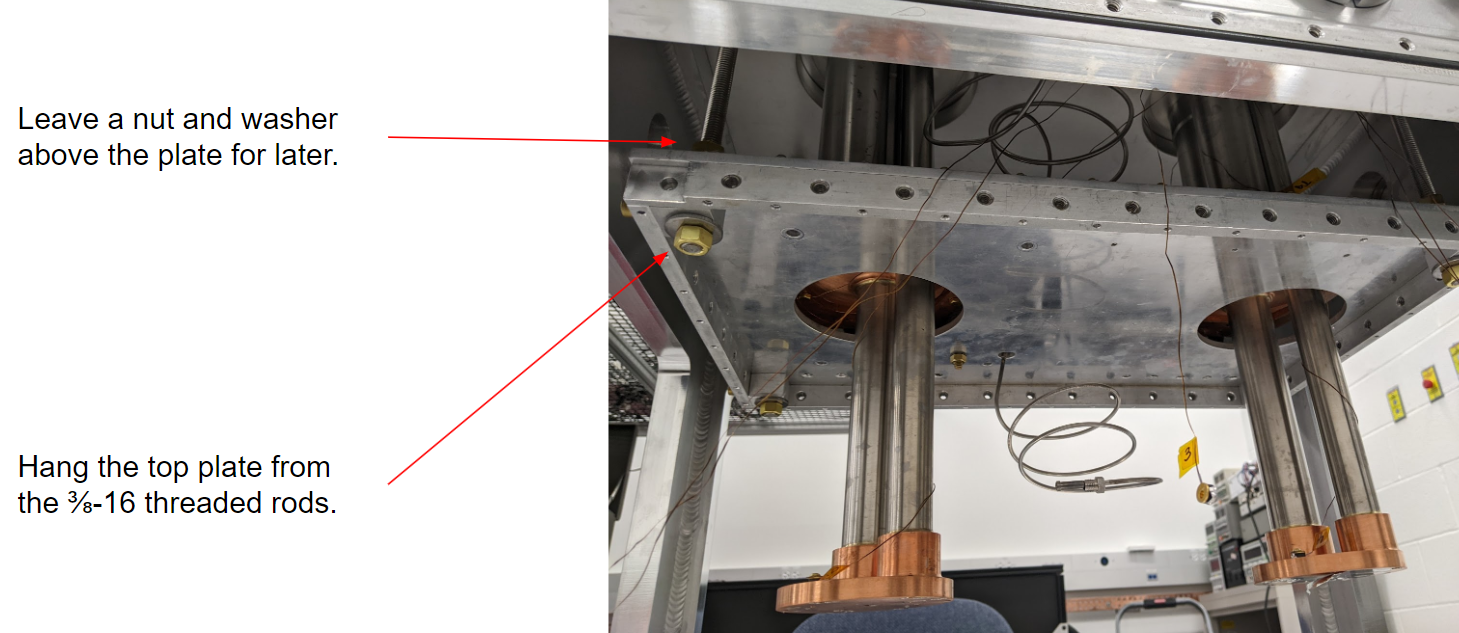
\includegraphics[width=\textwidth]{figs/todo/assembly/6E.png}
    \caption{Step 6E: top plate to threaded rods.}
    \label{beam_source_assembly_6E}
\end{figure}

\begin{figure}
    \centering
    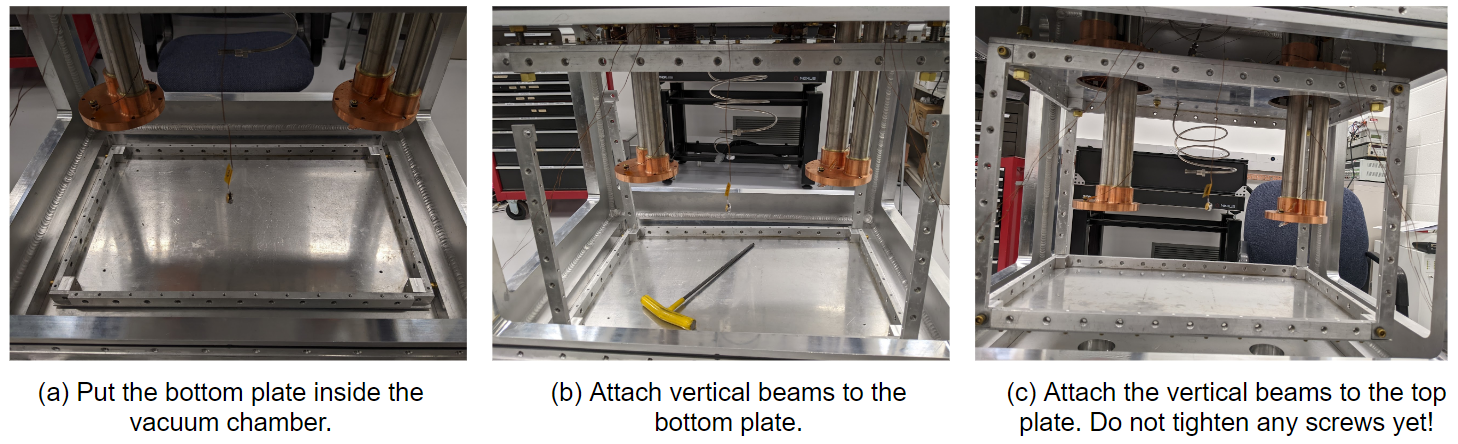
\includegraphics[width=\textwidth]{figs/todo/assembly/6G.png}
    \caption{Step 6G: Internal structure of 40K shield.}
    \label{beam_source_assembly_6G}
\end{figure}

\begin{figure}
    \centering
    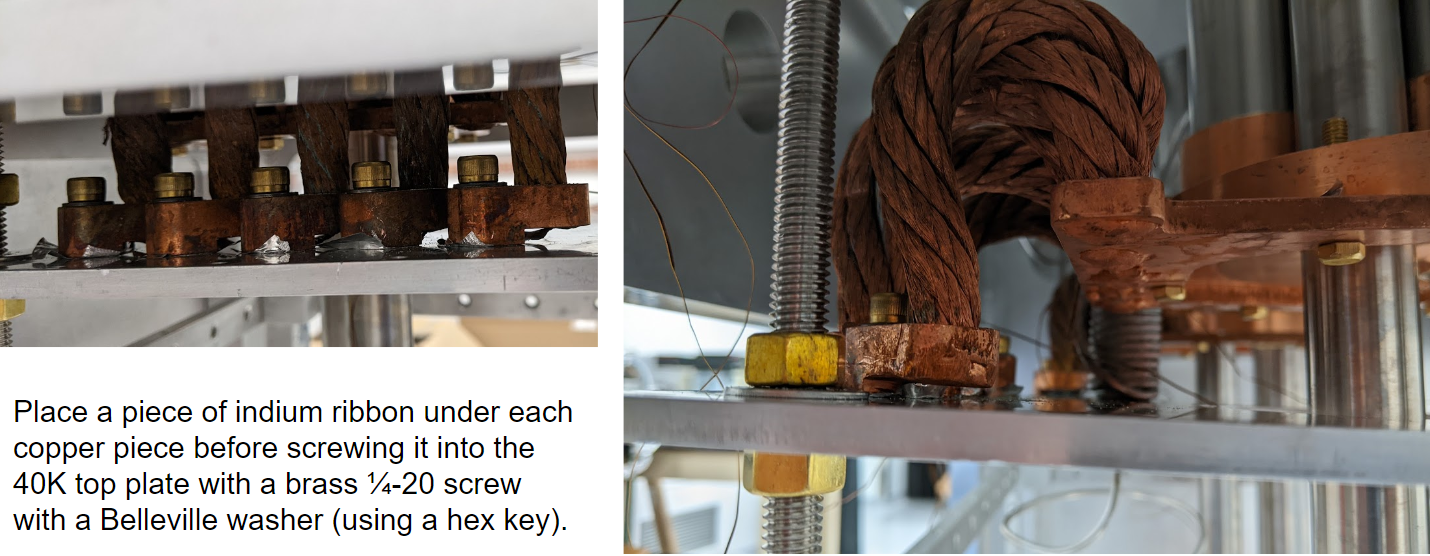
\includegraphics[width=\textwidth]{figs/todo/assembly/6H.png}
    \caption{Step 6H: Flexible heat links.}
    \label{beam_source_assembly_6H}
\end{figure}

\begin{figure}
    \centering
    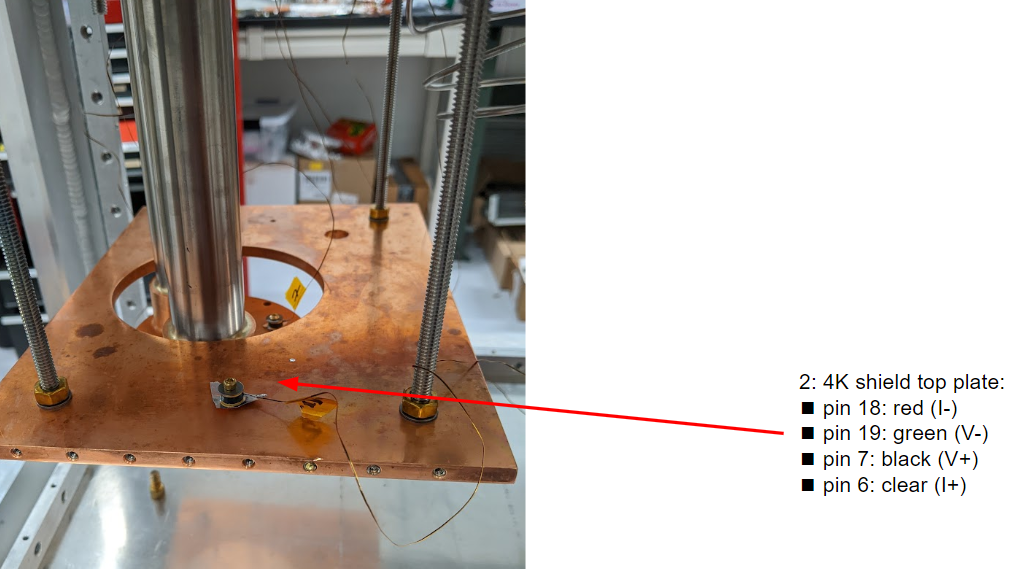
\includegraphics[width=\textwidth]{figs/todo/assembly/7A.png}
    \caption{Step 7A: 4K top plate + temperature sensor.}
    \label{beam_source_assembly_7A}
\end{figure}

\begin{figure}
    \centering
    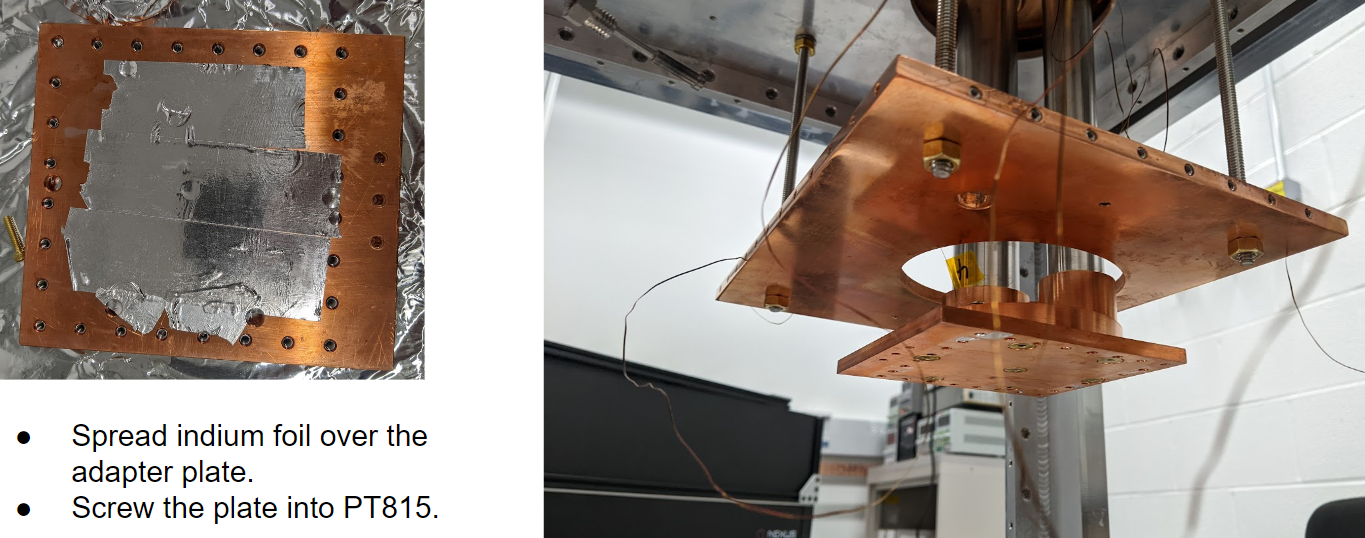
\includegraphics[width=\textwidth]{figs/todo/assembly/7B.png}
    \caption{Step 7B: PT815 adapter.}
    \label{beam_source_assembly_7B}
\end{figure}

\begin{figure}
    \centering
    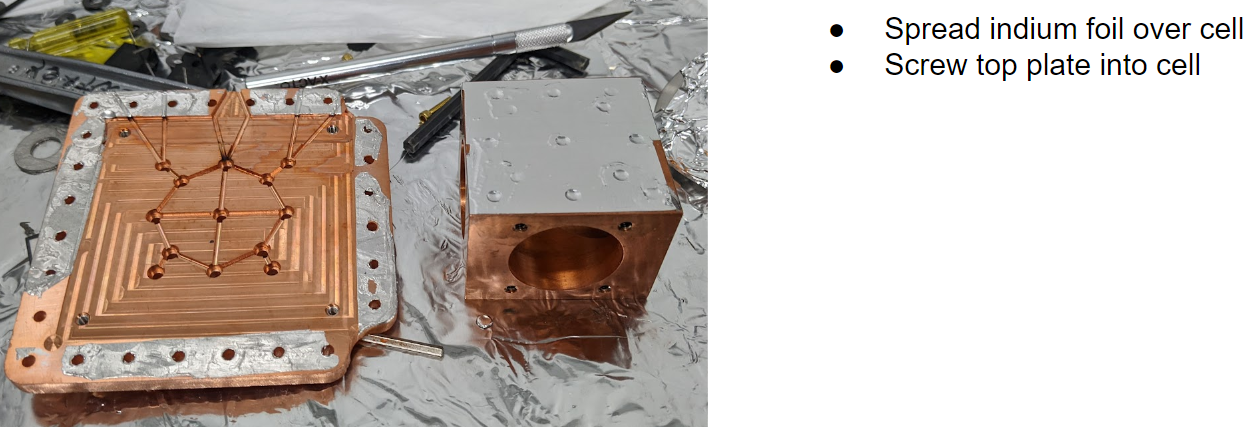
\includegraphics[width=\textwidth]{figs/todo/assembly/7C.png}
    \caption{Step 7C: Attach cell top plate to cell.}
    \label{beam_source_assembly_7C}
\end{figure}

\begin{figure}
    \centering
    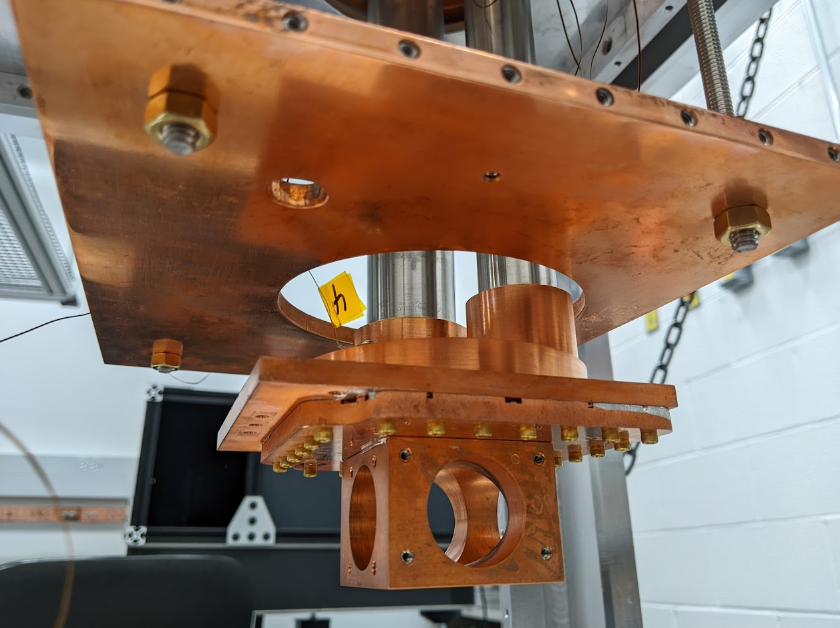
\includegraphics[width=.7\textwidth]{figs/todo/assembly/7D.png}
    \caption{Step 7D: Install cell onto PT815 adapter.}
    \label{beam_source_assembly_7D}
\end{figure}

\begin{figure}
    \centering
    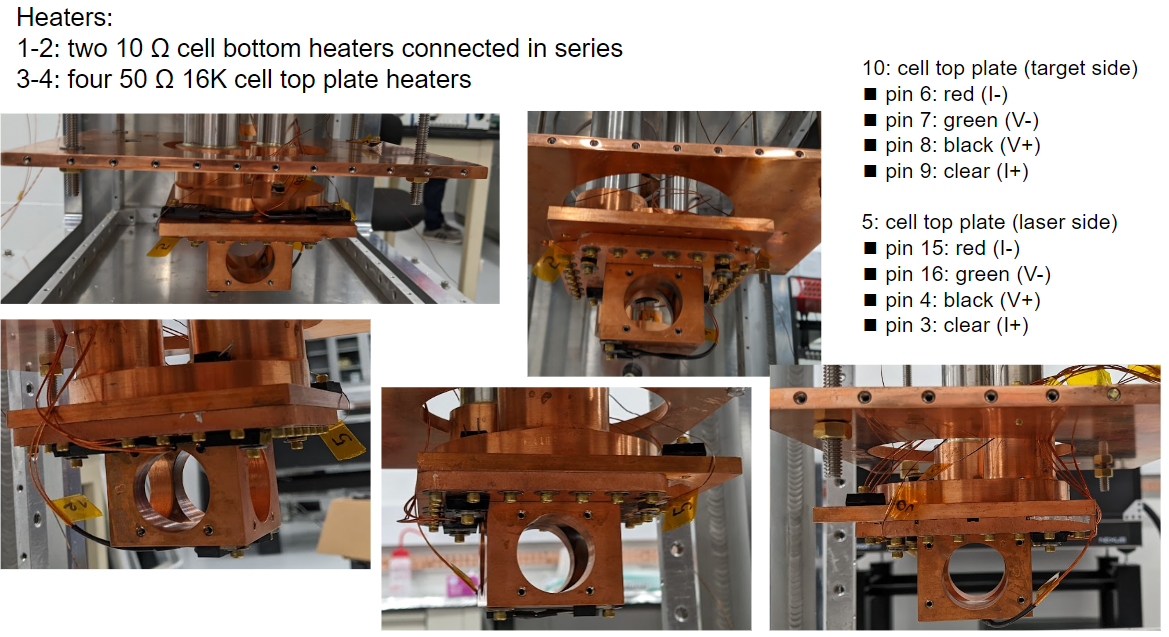
\includegraphics[width=\textwidth]{figs/todo/assembly/7E.png}
    \caption{Step 7E: Attach cell heaters \&\ thermometers.}
    \label{beam_source_assembly_7E}
\end{figure}

\begin{figure}
    \centering
    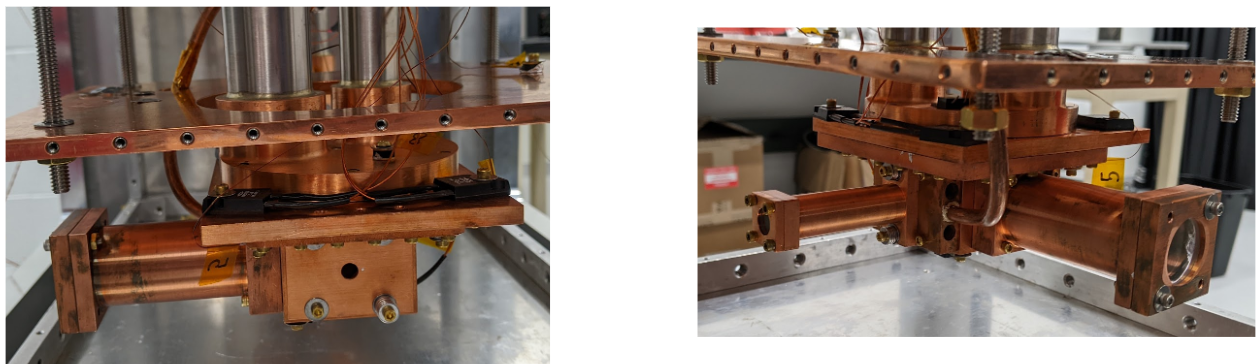
\includegraphics[width=\textwidth]{figs/todo/assembly/7F.png}
    \caption{Step 7F: Add snorkel, nozzle plate, input nozzle, back snorkel.}
    \label{beam_source_assembly_7F}
\end{figure}

\begin{figure}
    \centering
    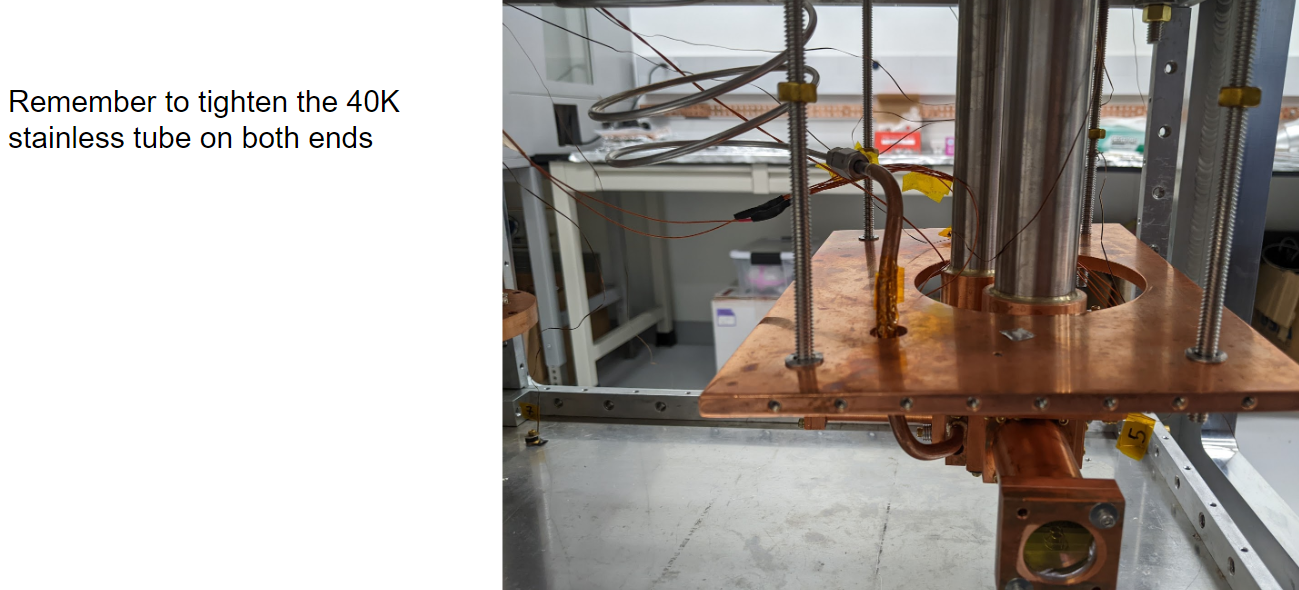
\includegraphics[width=\textwidth]{figs/todo/assembly/7G.png}
    \caption{Step 7G: Connect the neon line.}
    \label{beam_source_assembly_7G}
\end{figure}

\begin{figure}
    \centering
    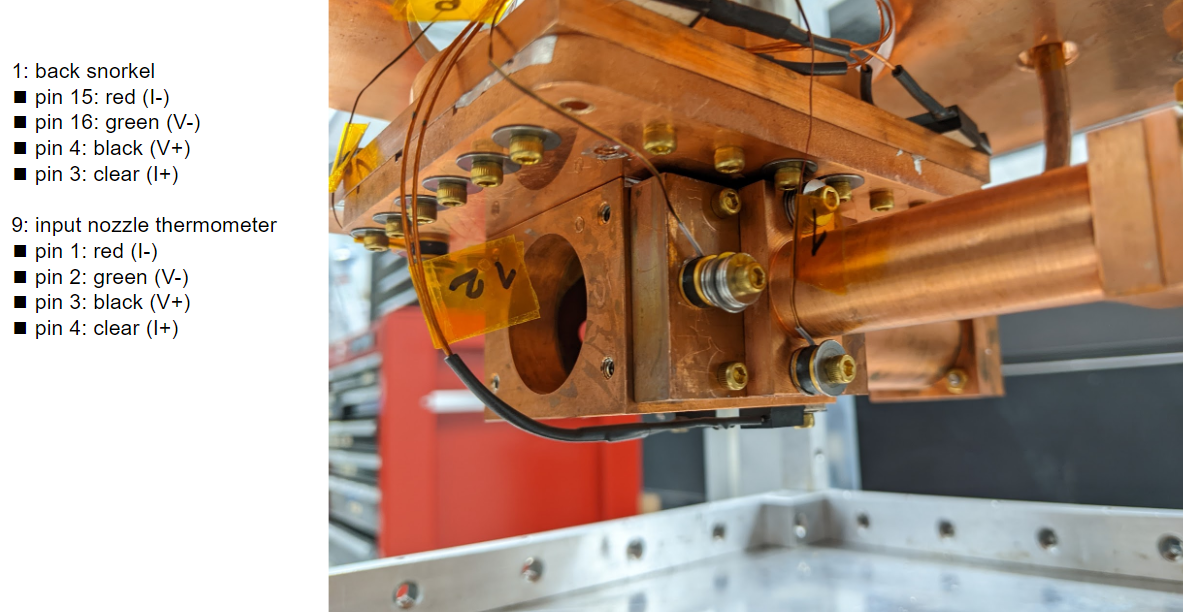
\includegraphics[width=\textwidth]{figs/todo/assembly/7H.png}
    \caption{Step 7H: Add remaining cell temperature sensors.}
    \label{beam_source_assembly_7H}
\end{figure}

\begin{figure}
    \centering
    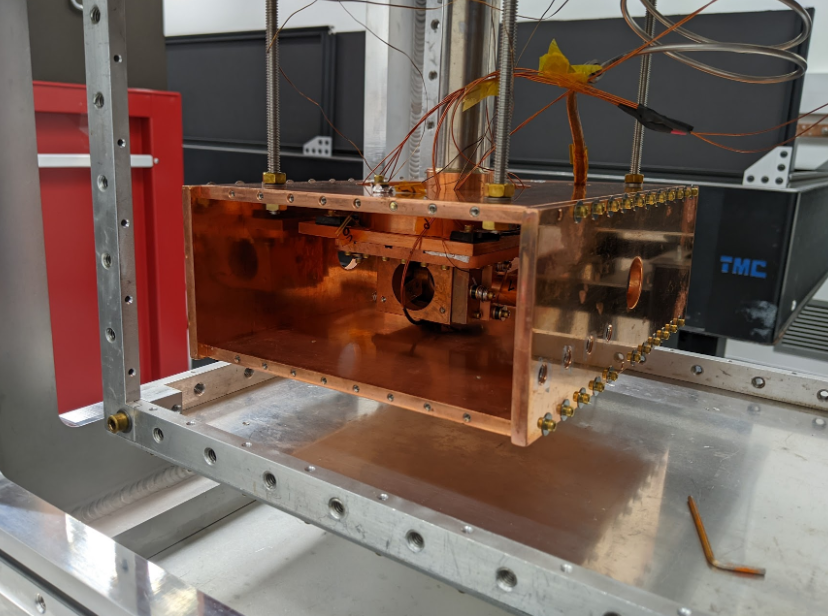
\includegraphics[width=.7\textwidth]{figs/todo/assembly/7I.png}
    \caption{Step 7I: Add 4K side plates, bottom plate.}
    \label{beam_source_assembly_7I}
\end{figure}

\begin{figure}
    \centering
    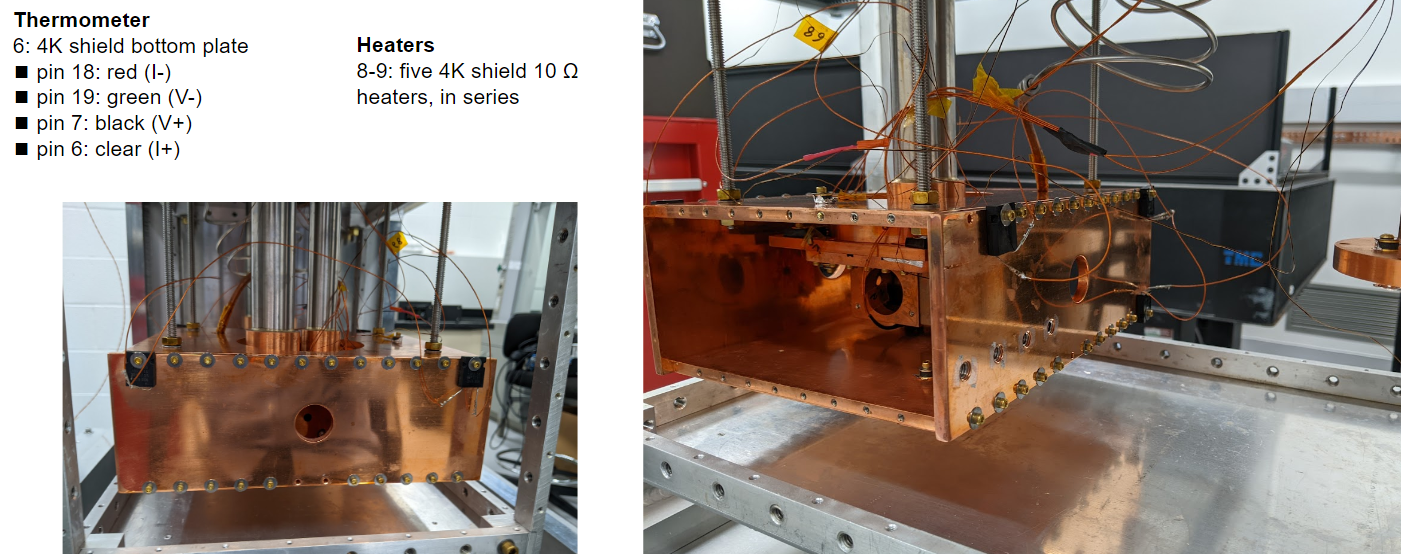
\includegraphics[width=\textwidth]{figs/todo/assembly/7J.png}
    \caption{Step 7J: Add 4K bottom thermometer, cell heaters.}
    \label{beam_source_assembly_7J}
\end{figure}
